%% TITLE	Physiological Fluid Mechanics, Summary 3

%% AUTHOR	BINGHUAN W LI (Dept. Chemical Eng/Bio Eng, Imperial)
%%          PETER Y XIE (Dept. Mech Eng, Stanford)

%% compiled in XeLaTeX with Tex Live version 2023.

%% This work is licensed under a Creative Commons Attribution-NonCommercial 4.0 International License.

%=====================================================
% Aug 30, 2024    
% 1. rename sec.2 to "Fluid Flow in a Rectangular Duct"
% 2. replace fig 2 and fig 3
% Sep 18, 2024    
% 1. add the left fig (shear strain) in fig 1
%=====================================================

\documentclass[a4paper]{article}
\def\NotesType{1}
\def\summaryNo{3}
\def\finalise{1}
%% TITLE	Physiological Fluid Mechanics, configuration

%% DATE		- Nov 19, 2023     create

%% AUTHOR	BINGHUAN W LI (Dept. Chemical Eng/Bio Eng, Imperial)
%%          PETER Y XIE (Dept. Mech Eng, Stanford)

%% compiled in XeLaTeX with Tex Live version 2023.

%% This work is licensed under a Creative Commons Attribution-NonCommercial 4.0 International License.

\usepackage[sfdefault]{arimo}
\usepackage[left=1.5cm, right=1.5cm, top=2cm, bottom=1.5cm]{geometry}
\usepackage{amsmath, amsfonts, amssymb, cancel}
\usepackage{unicode-math}
\setmathfont
    [    Extension = .otf,
         BoldFont = XITSMath-Bold,
    ]{XITSMath-Regular}

% % \DeclareMathSizes{10}{12}{10}{9}

% \usepackage{siunitx}
\usepackage{enumitem}
\usepackage{xcolor}
    \definecolor{linkcolour}{rgb}{0,0.2,0.6}
\usepackage{hyperref}
\hypersetup{
    colorlinks,
    breaklinks,
    urlcolor=linkcolour,
    linkcolor=linkcolour,
    citecolor=black,
    pdfauthor={Li, Binghuan W},
    }
\usepackage{graphicx, float}
\usepackage{framed}
\usepackage[export]{adjustbox}

\usepackage{fancyhdr}
    \pagestyle{fancy}
    \fancyhf{}
    \lhead{\textsc{Physiological Fluid Mechanics Summary \summaryNo}}
    \rhead{page \thepage}

\usepackage{tcolorbox}

\usepackage{tikz, circuitikz}

\usepackage{multicol}
    \setlength{\columnseprule}{1pt}

\usepackage{lscape}

\usepackage{booktabs}

\usepackage{pifont}

\setlength\parindent{0pt}

\begin{document}

\section{Fluid Viscosity}
For the Newtonian fluid, the dynamic viscosity $\mu$ $[\mathrm{Pa} \cdot \mathrm{s}]$ is a fixed constant; whereas for the non-Newtonian fluid, the viscosity varies with the shear stress $\tau$ $[\mathrm{Pa}]$ and shear rate $\dot{\gamma}$ $[1/\mathrm{s}]$.
\begin{figure}[H]
    \centering
    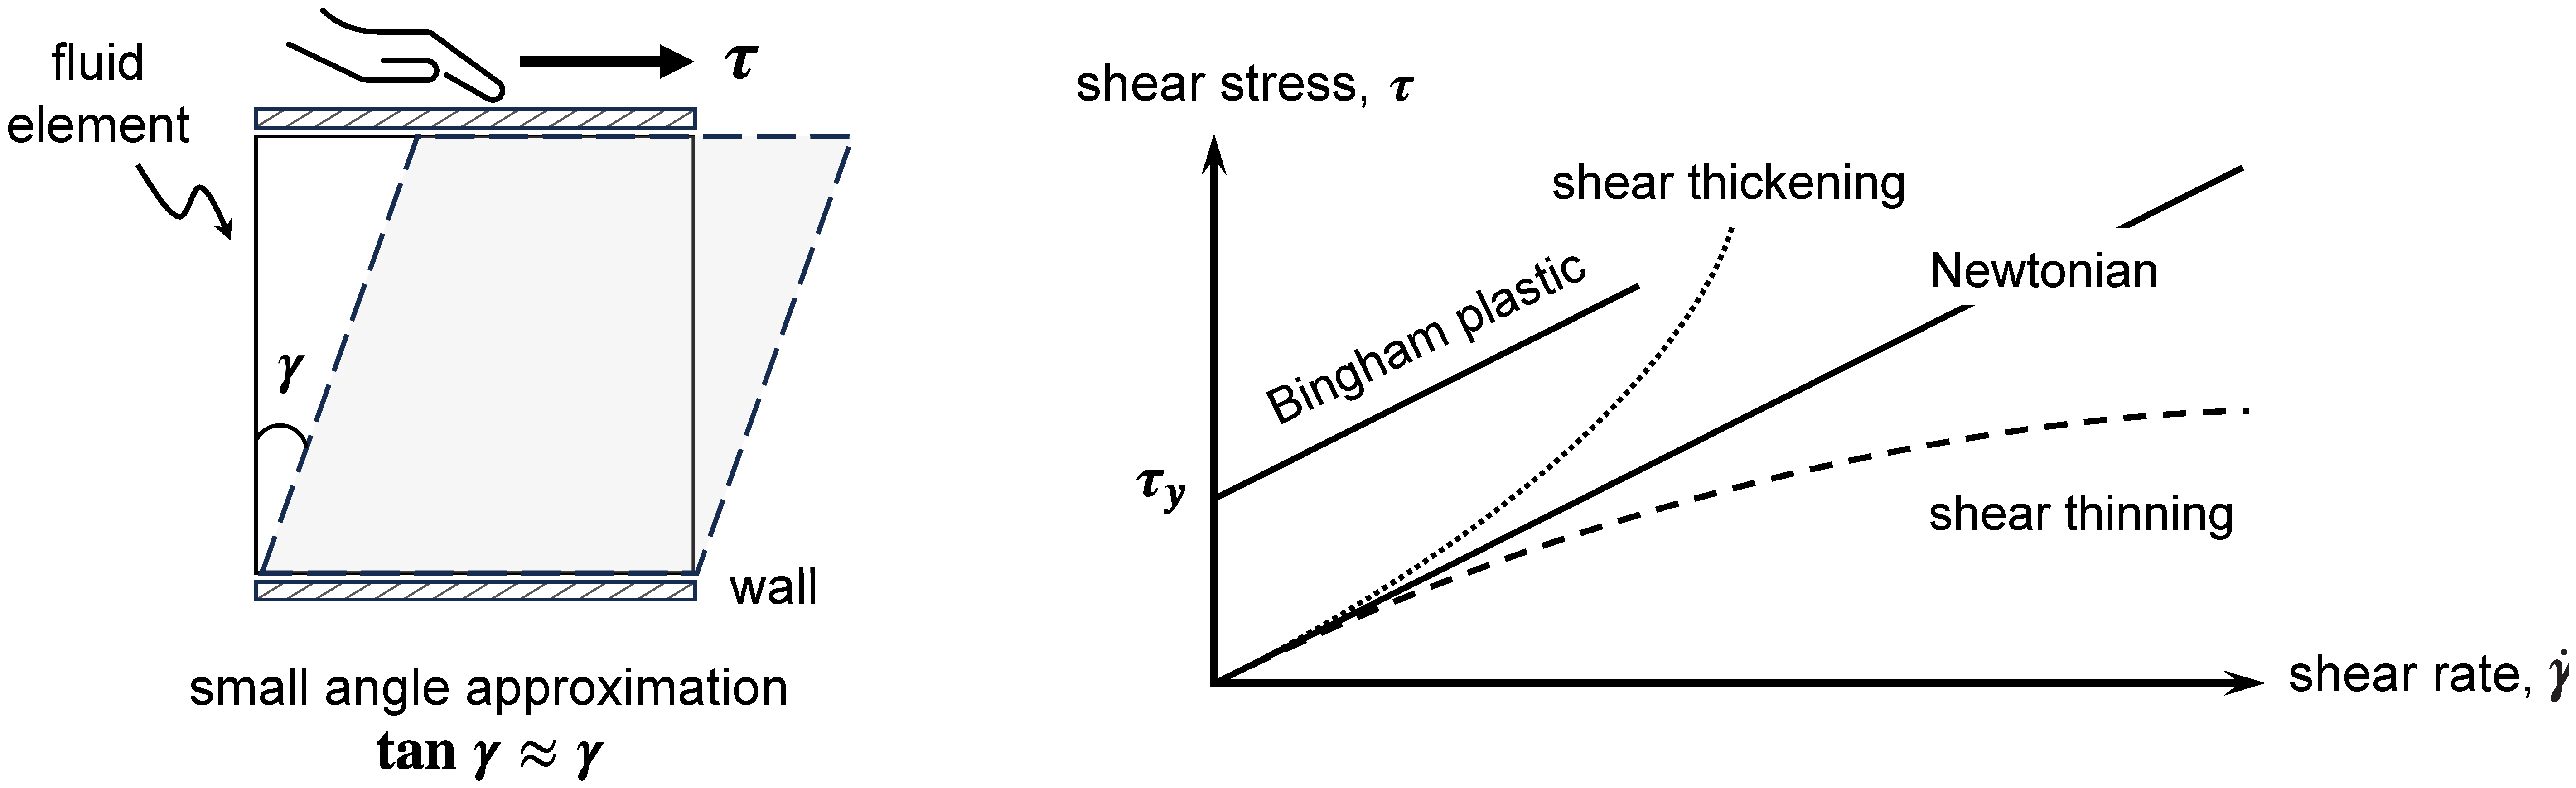
\includegraphics[width=\textwidth]{img/rheology.eps}
    \caption{Left: the concept of shear strain $\gamma$ in a simple shear flow; Right: the rheological behaviour of viscous fluids can be classified by the shear stress - shear rate ($\dot{\gamma} = \mathrm{d}\gamma / \mathrm{d}t$) relations.}
\end{figure}
\begin{itemize}
    \item Shear thickening: $\mu$ increases with shear rate - \textit{e.g.}, cornstarch paste;
    \item Shear thinning: $\mu$ decreases with shear rate - \textit{e.g.}, ketchup, blood;
    \item Bingham plastic: a yield stress $\tau_y$ impedes the fluid flow until $\tau > \tau_y$.
\end{itemize}
Although the blood is frequently modelled as a Newtonian fluid, it is shear thinning with yield (\textit{a.k.a.} Bingham pseudoplastic). The non-Newtonian behaviours of blood are due to the cell suspension (rather than the plasma), hence, the viscosity is Hematocrit-dependent.


\section{Flow in a Rectangular Duct}
Consider the flow in a rectangular duct (length $L$, width $w$, height $h$) in the Cartesian coordinate system (\autoref{fig:sqr_duct}).

\paragraph{Assumptions}
\begin{itemize}
    \item Fluid is homogeneous, incompressible and Newtonian with viscosity $\mu$ and density $\rho$;
    
    \item Flow has reached the steady state: $\partial \mathbf{u}/\partial t = 0$;
    
    \item Flow is fully developed along the $x$-direction: $\partial \mathbf{u} / \partial x = 0$;

    \item Zero velocity along the $y$- and $z$-directions: $v=0$, $w=0$;

    \item Negligible body force: $\mathbf{f} = 0$.
\end{itemize}

\paragraph{Boundary Conditions} Symmetrical flow profile at $y=0$ and $z=0$; no-slip condition at the wall $y=\pm h/2$, $z=\pm w/2$.

\paragraph{Aim} Analytically solve for the flow velocity in the $x$-direction.

\begin{figure}[h]
    \centering
    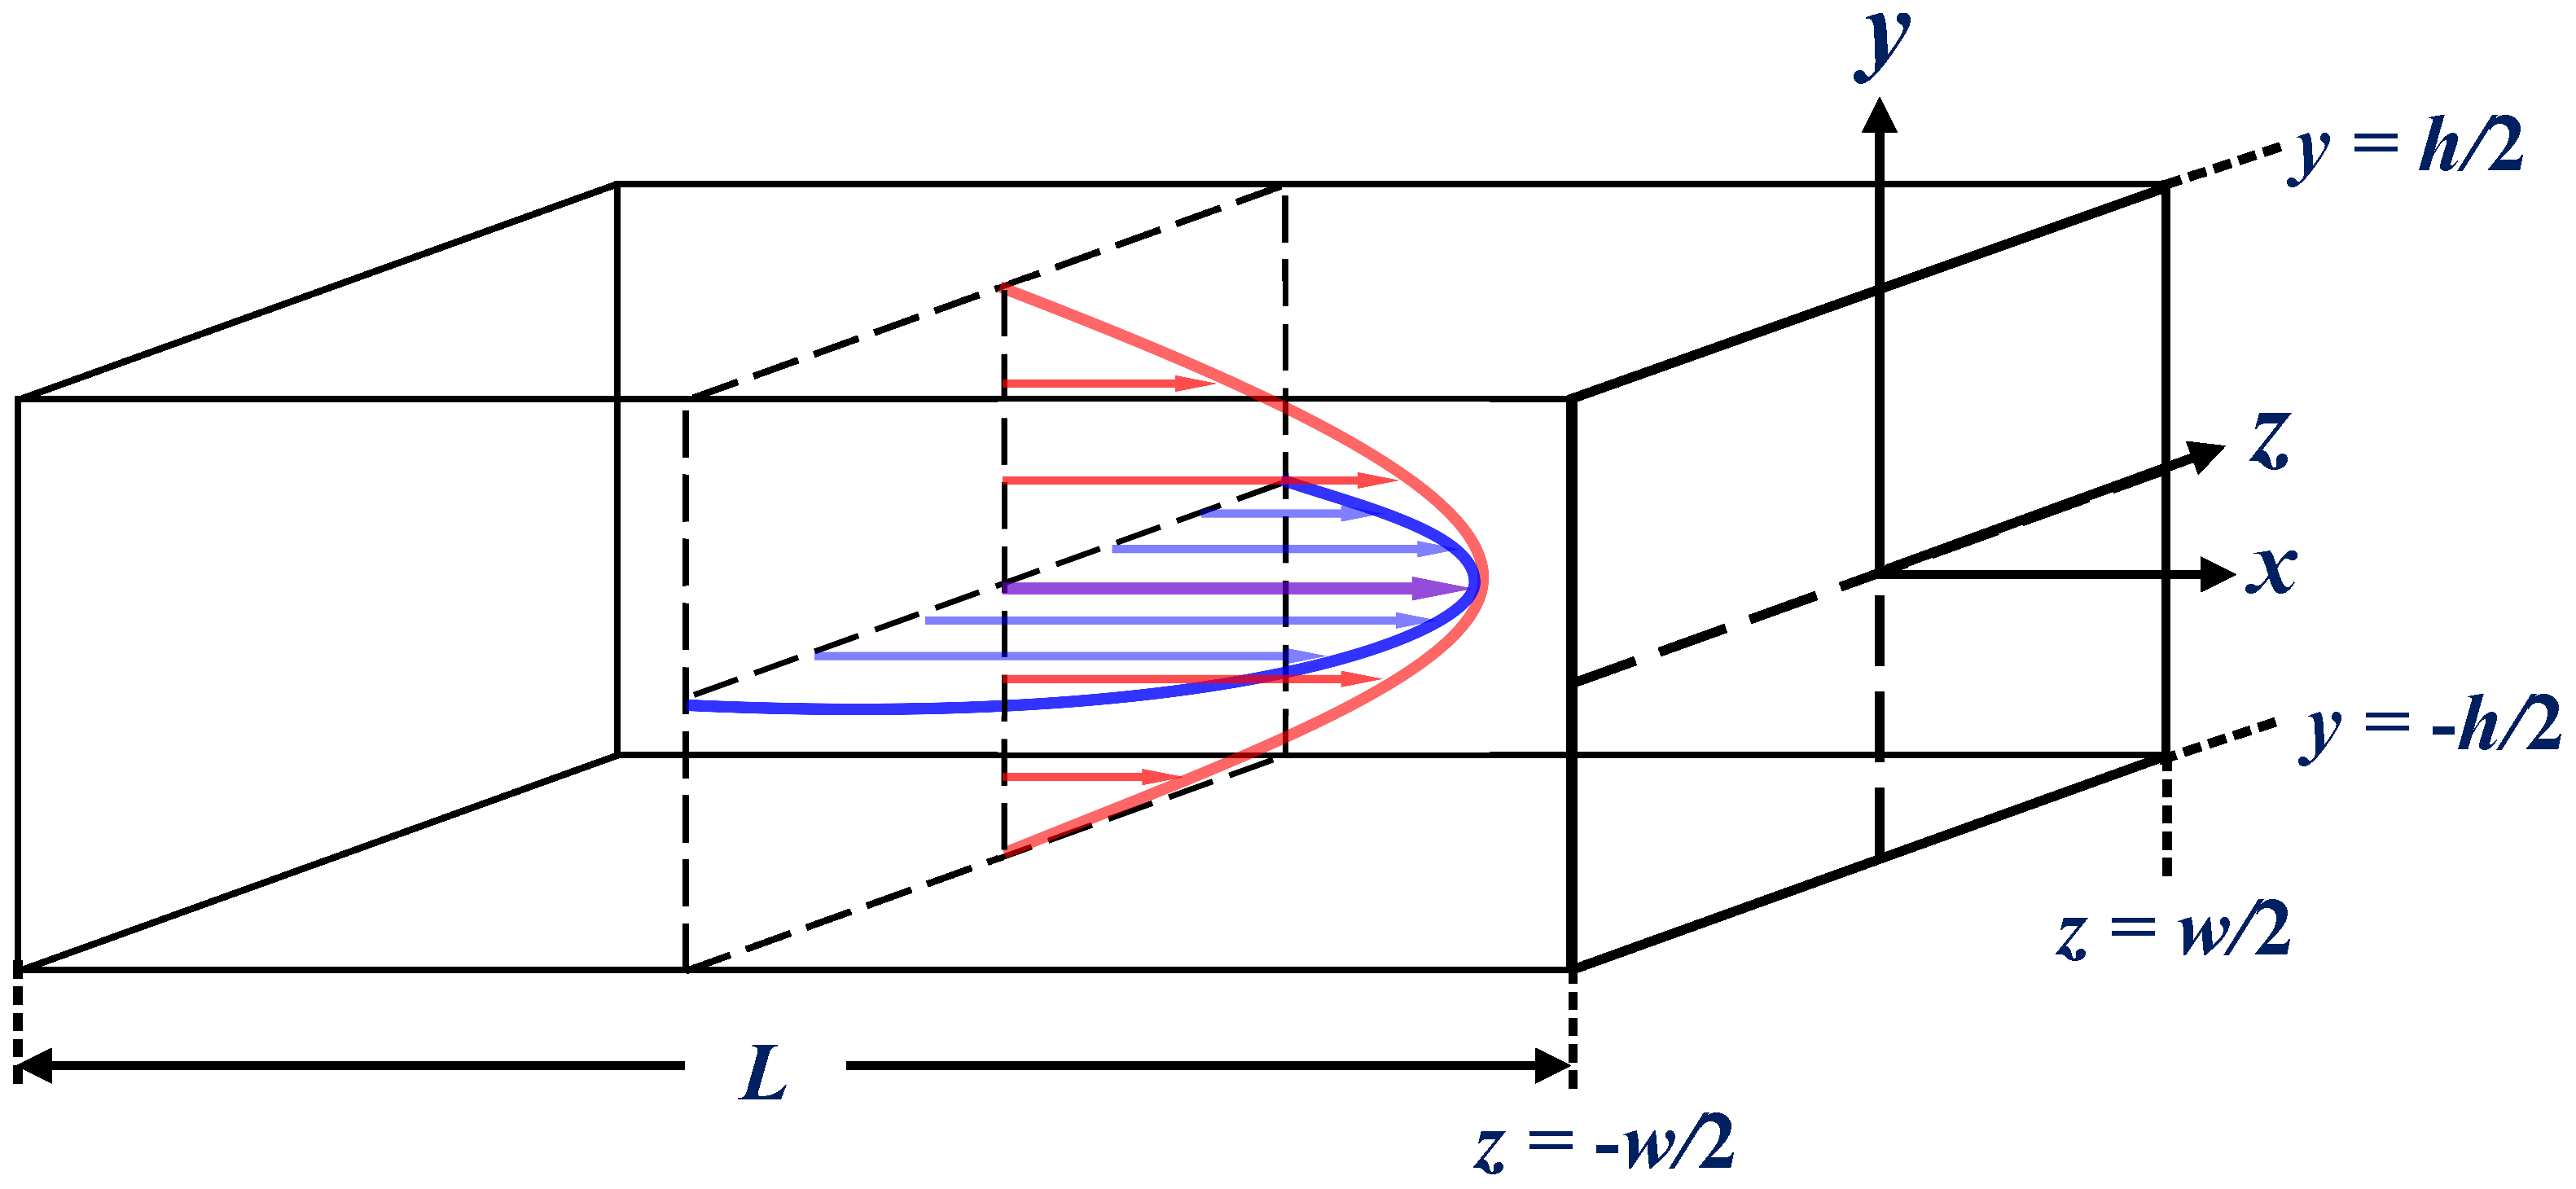
\includegraphics[width=.65\textwidth]{img/sqr_duct.eps}
    \caption{The schematic for the flow in a rectangular duct.}
    \label{fig:sqr_duct}
\end{figure}

\paragraph{Solution} The $x$-momentum equation is reduced to
\[
    0 = -\frac{\partial p}{\partial x} + \mu \bigg( \frac{\partial^2 u}{\partial y^2} + \frac{\partial^2 u}{\partial z^2} \bigg).
\]
Using separation of variables\footnote{for the full derivation, see the Supplementary slides posted on Blackboard}, the analytical solution of $u$ is
\[
    u = \frac{1}{2\mu} \frac{\partial p}{\partial x} \bigg[ y^2 - \bigg( \frac{h}{2} \bigg)^2 - \sum_{n=0}^\infty A_n \cos\bigg( \frac{\lambda_n y}{h/2} \bigg) \cosh \bigg(\frac{\lambda_n z}{h/2} \bigg) \bigg], \quad \text{where} \ A_n = \frac{h^2 (-1)^n}{\lambda_n^3 \cosh \frac{\lambda_n w}{h}}, \quad \lambda_n = \frac{(2n+1)\pi}{2}.
\]
Integrating $u$ over the area, the flux $Q$ can be expressed as
\[
    Q 
    = \frac{\partial p}{\partial x} \frac{wh^3}{12\mu} \bigg[ 6\bigg(\frac{h}{w}\bigg) \sum_{n=0}^{\infty} \lambda_n^{-5} \tanh \bigg( \frac{\lambda_n w}{h} \bigg) - 1 \bigg] 
    \quad {\color{red}\approx} \quad \frac{\partial p}{\partial x} \frac{wh^3}{12\mu} \bigg[ 1 - 0.6274 \bigg( \frac{h}{w} \bigg) \bigg].
\]
Finally, by $Q = \Delta p/R$, the flow resistance is
\[
    R = \frac{\Delta p}{Q} = \frac{12 \mu L}{wh^3 \bigg[ 1 - 0.6274 \bigg( \dfrac{h}{w} \bigg) \bigg]}.
\]

\section{Womersley Flow}
\paragraph{Motivation}  To approximate the pulsatility nature of the flow in the cardiovascular system.


\paragraph{Assumptions}
\begin{itemize}
    \item Fluid is homogeneous, incompressible and Newtonian with viscosity $\mu$ and density $\rho$;

    \item Flow in a long straight tube, with a perfect circular cross-section at radius $a$;
    
    \item Axisymmetric along the $\theta$-axis: $\partial/\partial \theta=0$; 

    \item The flow is fully developed along the $z$-axis: $\partial \mathbf{u} / \partial z=0$; 

    \item No swirls: $u_{\theta}=0$;

    \item No velocity along the radial direction: $u_r = 0$;

    \item Negligible body force: $\mathbf{f} = 0$.
\end{itemize}

\vspace{-.5cm}
\begin{figure}[H]
    \centering
    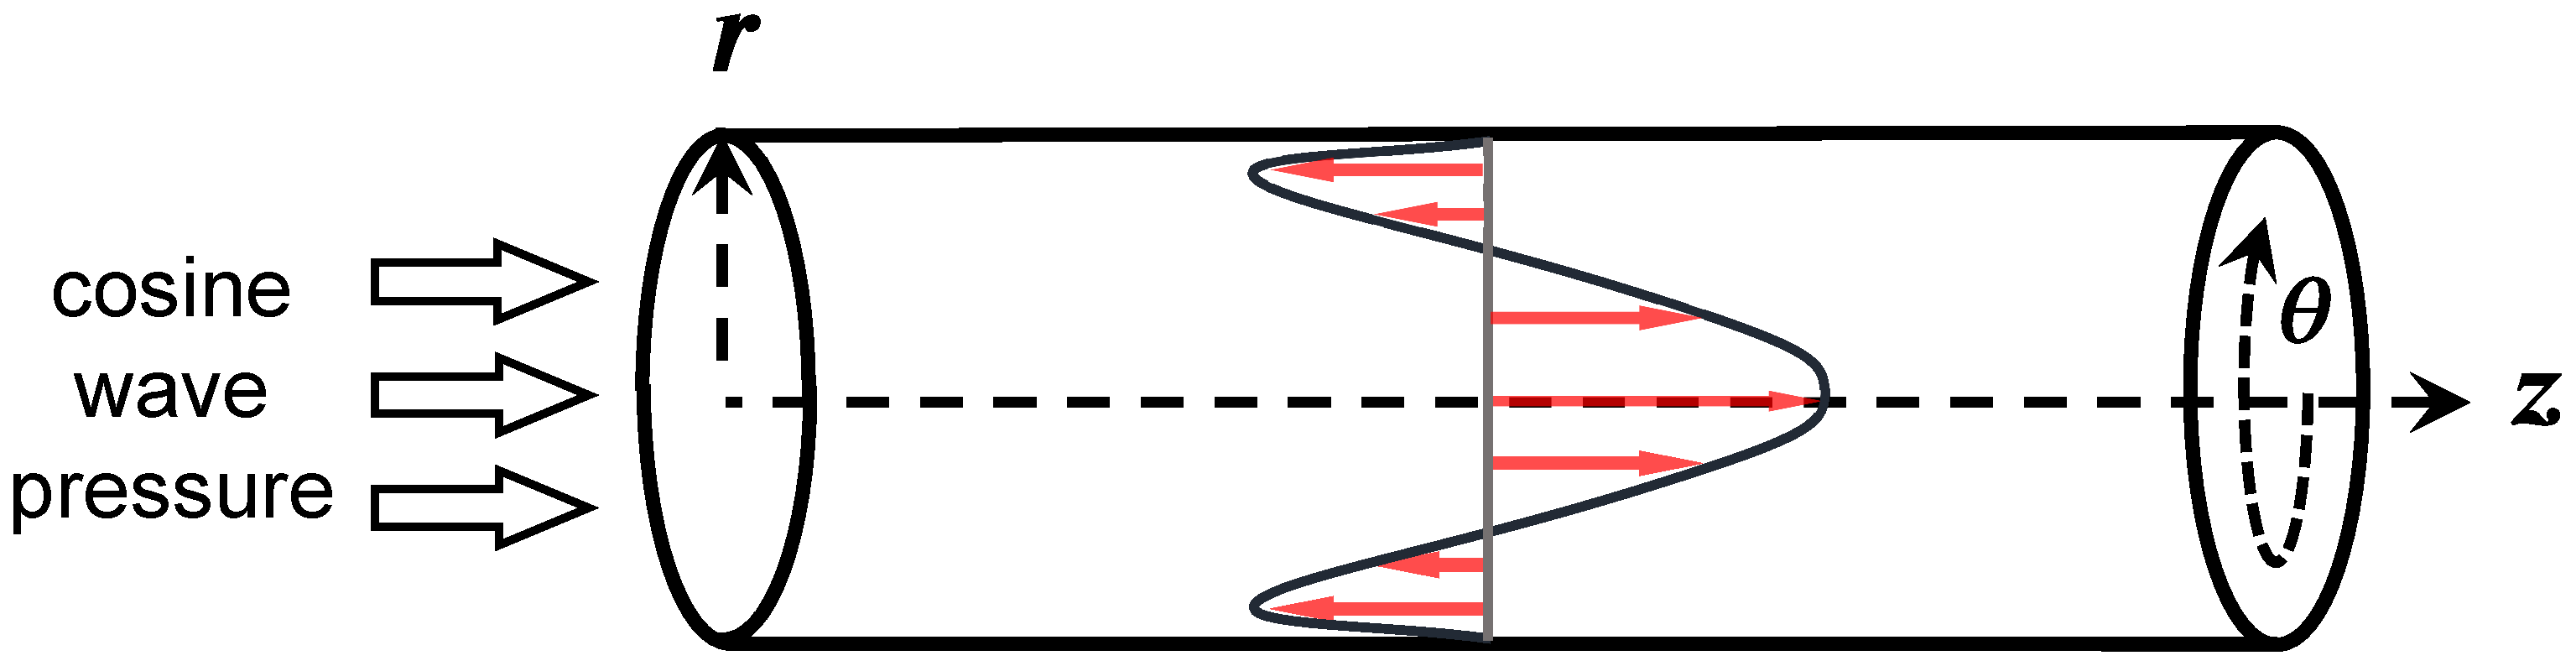
\includegraphics[width=.7\textwidth]{img/wo-pipe.eps}
    \caption{The schematic of the Womersley flow in a pipe.}
\end{figure}

\paragraph{Boundary Conditions} No-slip condition on the wall, parabolic condition as Poiseuille flow.

\paragraph{Solution Procedure}
\begin{enumerate}[label=\underline{\textbf{Step \arabic*}}]
    \item The $z$-momentum equation
    \[
        \rho \bigg(\frac{\partial u_{z}}{\partial t} + \cancelto{0}{u_{r} \frac{\partial u_{z}}{\partial r}} + \cancelto{0}{\frac{u_{\theta}}{r}\frac{\partial u_{z}}{\partial \theta}} + \cancelto{0}{u_{z}\frac{\partial u_{z}}{\partial z}} \bigg) = -\frac{\partial p}{\partial z} + \mu \bigg[ \frac{1}{r}\frac{\partial}{\partial r} \bigg(r \frac{\partial u_{z}}{\partial r}\bigg) + \cancelto{0}{\frac{1}{r^{2}} \frac{\partial^{2} u_{z}}{\partial \theta^{2}}} + \cancelto{0}{\frac{\partial^{2} u_{z}}{\partial z^{2}}} \bigg] + \cancelto{0}{\rho f_{z}}
    \]
    \[
        \Rightarrow \quad \rho \frac{\partial u_z}{\partial t} = -\frac{\partial p}{\partial z} + \mu \frac{1}{r} \frac{\partial}{\partial r} \bigg(r\frac{\partial u_z}{\partial r} \bigg).
    \]
    Assume the pressure gradient is sinusoidal: $\displaystyle \partial p / \partial z = \frac{G_0}{2}e^{i\omega t}$, and following the sinusoidal $z$-velocity: $u_z = U(r) e^{i\omega t}$:
    \[
        \bigg[ i\omega U \rho + \frac{G_0}{2} - \mu \frac{1}{r}\frac{\partial}{\partial r} \bigg(r\frac{\partial U}{\partial r}\bigg) \bigg] e^{i\omega t} = 0
        \quad \xrightarrow[]{\text{2\textsuperscript{nd}-order ODE}} \quad
        \frac{\partial^2 U}{\partial r^2} + \frac{1}{r} \frac{\partial U}{\partial r} - \frac{i\omega \rho}{\mu} U = - \frac{G_0}{2\mu}.
    \]

    \item The full solution of $U(r)$ involves a complementary function, which is formulated with the Bessel function of the 1\textsuperscript{st} kind at 0\textsuperscript{th} order, $J_0$; also the particular integral, $U_{pi} = -G_0 / 2i\omega \rho$:
    \[\
        U(r) = \frac{iG_{0}}{2\omega \rho}\bigg[ 1- \frac{J_{0}(i^{3/2}\alpha \frac{r}{a})}{J_{0}(i^{3/2}\alpha)} \bigg],
        \quad \text{with} \quad 
        J_0(s) = \sum_{k=0}^{+\infty} \frac{(-1)^k}{k!k!}\bigg(\frac{s}{2}\bigg)^{2k},
    \]
    and $\alpha$ denotes the non-dimensional \textbf{Wormersley number}: $\displaystyle \alpha = a \sqrt{\frac{\omega \rho}{\mu}} = a \sqrt{\frac{\omega}{\nu}}$.
    
    \item To recover $u_z$ from $U(r)$:
    \[
        u_{z}(r,t) 
        = \frac{i}{\omega \rho} \frac{\partial p}{\partial z} \bigg[ 1- \frac{J_{0}(i^{3/2}\alpha \frac{r}{a})}{J_{0}(i^{3/2}\alpha)} \bigg] 
        = \frac{iG_{0}}{2\omega \rho}\bigg[ 1- \frac{J_{0}(i^{3/2}\alpha \frac{r}{a})}{J_{0}(i^{3/2}\alpha)} \bigg] e^{i\omega t}
    \]
    Ostensibly, this solution is defined in the complex domain; but for simplicity, we only consider the real part to interpret its physical meaning.
\end{enumerate}

\paragraph{Extended Properties}
\begin{enumerate}
    \item  Wall shear stress: 
    \[
        \tau_{rz} = \mu \frac{\partial u_{z}}{\partial r} = \mu \Re\bigg\{ -\frac{a}{i^{3/2}\alpha} \bigg( \frac{J_{1}(i^{3/2}\alpha)}{J_{0}(i^{3/2}\alpha)} \bigg) \frac{\partial p}{\partial z} \bigg\}, 
        \quad \text{with} \quad 
        J_1(s) = -\frac{\partial J_0(s)}{\partial s}.
    \]

    \item Volume flow rate: 
    \[
        Q(t) = \int_{0}^{a} 2\pi r u_{z} \mathrm{d}r = \Re\bigg\{ -\frac{\pi a^{4}}{i \mu \alpha^{2}} \bigg( 1 - \frac{2J_{1}(i^{3/2}\alpha)}{\alpha i^{3/2} J_{0}(i^{3/2}\alpha)} \bigg) \frac{\partial p}{\partial z} \bigg\}.
    \]
\end{enumerate}

\paragraph{The Wormersley Number}
The Wormersley number $\alpha$ is the ratio between unsteady inertia force and viscous force.
\begin{itemize}
    \item $\alpha \leq 1 $: \textbf{Quasi-steady}, the velocity profile is basically scaled Poiseuille flow, mainly observed in the microvasculatures (\textit{e.g.}, capillaries, venules);
    \item $\alpha > 1 $: \textbf{Oscillatory}, the velocity profile is balanced between viscous forces at the wall and inertial forces in the centre. Common in large arteries (\textit{e.g.}, ascending aorta, carotid artery).
\end{itemize}

\begin{figure}[H]
    \centering
    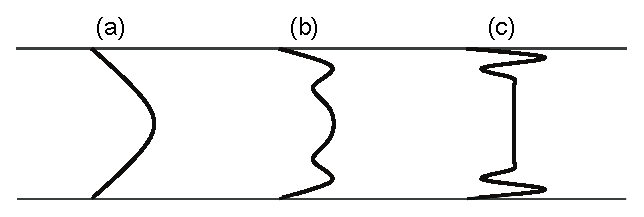
\includegraphics[width=.55\textwidth]{img/wo_plot.eps}
    \caption{Womersley flow profiles. (a) Low $\alpha$ (viscous dominates), (b) intermediate $\alpha$, (c) high $\alpha$ (inertia dominates).}
\end{figure}


\vfill
{\small \color{gray}Drafted by B. Li, H. El Nashar, and C. H. Yap,  \today}
% \thispagestyle{empty}
\newgeometry{margin=1.8cm}
\mbox{}
\vfill    
\begin{figure}[H]
    \includegraphics[right]{images/by-nc.eps}
\end{figure}
\textit{This work is licensed under a Creative Commons Attribution-NonCommercial 4.0 International License.}


\end{document}